\documentclass{article}
\usepackage[utf8]{inputenc}
% \usepackage{l3backend}
% \usepackage{fontspec}
\usepackage[usenames,svgnames]{xcolor}
% \usepackage{xunicode}
\usepackage{amssymb}
% Page setup
\usepackage[a4paper,landscape,margin=2cm]{geometry}
\usepackage{amsmath}
% \newfontfamily\ubuntumono{Ubuntu Mono}
% Typography
\usepackage[scaled]{helvet}
\renewcommand{\familydefault}{\sfdefault}
%\let\familydefault\sfdefault

\usepackage{tikz,pgfplots,tikz-layers,tikzpeople}
\usetikzlibrary{positioning,arrows,intersections,calc,fit,backgrounds,shapes,matrix}

\definecolor{colorbook}     {RGB}{ 79,142,209}
\definecolor{colorprofile}  {RGB}{143,232,186}
\definecolor{colorperson}   {RGB}{190, 22, 34}

\definecolor{colorgray}     {RGB}{150,150,150}
\definecolor{colorpod}      {RGB}{199,212,104}
\definecolor{colorpod2}      {RGB}{227, 222, 171}
\definecolor{colorfile}     {RGB}{ 79,142,209}
\definecolor{colorsummary}  {RGB}{143,232,186}
\definecolor{colortext}     {RGB}{ 29, 29, 27}
\definecolor{colorkey}      {RGB}{129, 29, 27}
\definecolor{colorclient}   {RGB}{190, 22, 34}
\definecolor{colorrepeat}   {RGB}{255,240,240}
\definecolor{colorwhite}    {RGB}{255,255,255}

\makeatletter
\pgfdeclareshape{datastore}{
  \inheritsavedanchors[from=rectangle]
  \inheritanchorborder[from=rectangle]
  \inheritanchor[from=rectangle]{center}
  \inheritanchor[from=rectangle]{base}
  \inheritanchor[from=rectangle]{north}
  \inheritanchor[from=rectangle]{north east}
  \inheritanchor[from=rectangle]{east}
  \inheritanchor[from=rectangle]{south east}
  \inheritanchor[from=rectangle]{south}
  \inheritanchor[from=rectangle]{south west}
  \inheritanchor[from=rectangle]{west}
  \inheritanchor[from=rectangle]{north west}
  \backgroundpath{
    %  store lower right in xa/ya and upper right in xb/yb
    \southwest \pgf@xa=\pgf@x \pgf@ya=\pgf@y
    \northeast \pgf@xb=\pgf@x \pgf@yb=\pgf@y
    \pgfpathmoveto{\pgfpoint{\pgf@xa}{\pgf@ya}}
    \pgfpathlineto{\pgfpoint{\pgf@xb}{\pgf@ya}}
    \pgfpathmoveto{\pgfpoint{\pgf@xa}{\pgf@yb}}
    \pgfpathlineto{\pgfpoint{\pgf@xb}{\pgf@yb}}
 }
}
\makeatother
\tikzset{every picture/.style={/utils/exec={\sffamily\itshape}}}




\begin{document}
\pagestyle{empty}


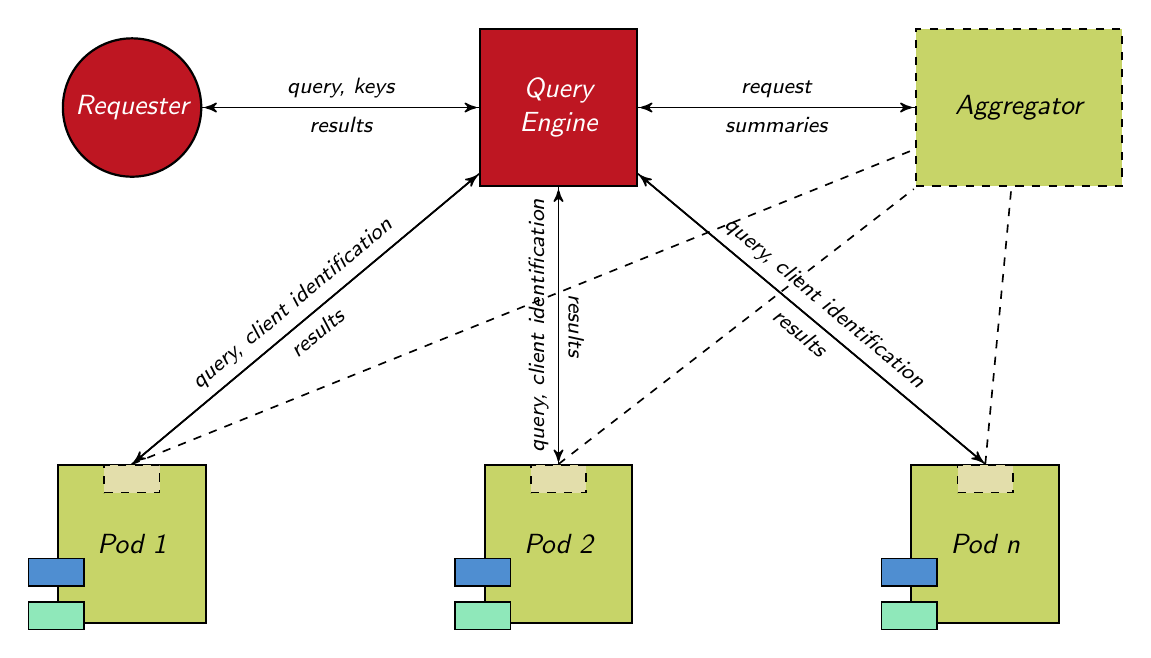
\begin{tikzpicture}[
    node distance = 10em, auto, thick,
    title/.style={text=colortext,font={\Large\itshape}},
    person/.style={text=colorwhite,font={\Large\bfseries}},
    code/.style={text=colortext,font={}},
        % Client
    key/.style={text=colorkey,font={\tiny\itshape}},
    every matrix/.style={ampersand replacement=\&,column sep=2cm,row sep=2cm ,
        nodes in empty cells},
    matrixstyle/.style={
        matrix of nodes,
        nodes in empty cells,
        column sep      = -\pgflinewidth,
        row sep         = -\pgflinewidth,
        nodes={%
            inner sep=0mm,outer sep=0pt,
            minimum size=5mm,
            text height=\ht\strutbox,text depth=\dp\strutbox,
            draw
          }},
    source/.style={draw,thick,fill=yellow!20,inner sep=.3cm},
    db/.style={draw,thick,fill=yellow!20},
    process/.style={draw,thick,circle,fill=colorfile},
    sink/.style={source,inner sep=.5cm, minimum height=2cm},
    pod/.style={draw,thick,rectangle,fill=colorpod,inner sep=.5cm, minimum height=2cm},
    datastore/.style={draw,very thick,shape=datastore,inner sep=.3cm},
    dots/.style={gray,scale=2},
    to/.style={->,>=stealth',shorten >=1pt,semithick,font=\sffamily\footnotesize},
    every node/.style={align=center}]

  % % Position the nodes using a matrix layout
  % \& \node[datastore] (buffer) {buffer};  \& \\

  \node[draw,fill=colorclient,text=colorwhite,circle,minimum size=1em] (REQUESTER){Requester};
  \node[sink, fill=colorclient,text=colorwhite, right=of REQUESTER] (FE) {Query \\ Engine};
  \node[sink, fill=colorpod,dashed, right = of FE] (IAM) [align=left] {Aggregator};
  \node[pod, below = of FE] (POD2) {Pod 2};
  \node[pod, left = of POD2] (POD1) {Pod 1};
  \node[pod, right = of POD2] (POD3) {Pod n};
  % \node[title,font=\sffamily\footnotesize, below=0.5em of POD1] (KPOD1) {$K_1^{Pod_1}\dots K_n^{Pod_1}$};
  % \node[title,font=\sffamily\footnotesize, below=0.5em of POD2] (KPOD2) {$K_1^{Pod_2}\dots K_n^{Pod_2}$};
  % \node[title,font=\sffamily\footnotesize, below=0.5em of POD3] (KPOD3) {$K_1^{Pod_n}\dots K_n^{Pod_n}$};
  % \node[title, below=1em of POD3] (KPOD2) {};


  \draw[to] (REQUESTER) -- node[midway,above] {query, keys}  (FE);
  \draw[to] (FE) -- node[midway,below] {results} (REQUESTER);

  \draw[to] (IAM) -- node[midway,above] {request} (FE);
  \draw[to] (FE) -- node[midway,below] {summaries} (IAM);

  \draw[to,>=stealth',shorten >=1pt,semithick,font=\sffamily\footnotesize] (POD1.north) -- node[midway,above,sloped] {query, client identification} (FE);
  \draw[to,>=stealth',shorten >=1pt,semithick,font=\sffamily\footnotesize] (FE) -- node[midway,below,sloped] {results} (POD1.north);


  \draw[to,>=stealth',shorten >=1pt,semithick,font=\sffamily\footnotesize] (POD2.north) -- node[midway,above,sloped] {query, client identification} (FE);
  \draw[to,>=stealth',shorten >=1pt,semithick,font=\sffamily\footnotesize] (FE) -- node[midway,above,sloped] {results} (POD2.north);

  \draw[to,>=stealth',shorten >=1pt,semithick,font=\sffamily\footnotesize] (POD3.north) -- node[midway,above,sloped] {query, client identification} (FE);
  \draw[to,>=stealth',shorten >=1pt,semithick,font=\sffamily\footnotesize] (FE) -- node[midway,below,sloped] {results} (POD3.north);


  \draw[-,>=stealth',shorten >=1pt,semithick,dashed,font=\sffamily\footnotesize] (POD1.north) -- node[midway,sloped] {} (IAM);
  \draw[-,>=stealth',shorten >=1pt,semithick,dashed,font=\sffamily\footnotesize] (POD2.north) -- node[midway,sloped] {} (IAM);
  \draw[-,>=stealth',shorten >=1pt,semithick,dashed,font=\sffamily\footnotesize] (POD3.north) -- node[midway,sloped] {} (IAM);

  \begin{scope}[on above layer]
    \node[fill=colorfile, draw, semithick,below left=0.5em and -1em of POD1.west, rectangle,minimum width=2em,minimum height=1em] (blue1) {};
    \node[fill=colorsummary, draw, semithick,rectangle,below= 0.5em of blue1, minimum width=2em, minimum height=1em] (green1) {};
    \node[fill=colorpod2,  dashed, draw, semithick,rectangle,below = 0em of POD1.north, minimum width=2em, minimum height=1em] (ac1) {};
    \node[fill=colorfile, draw, semithick,below left=0.5em and -1em of POD2.west, rectangle,minimum width=2em,minimum height=1em] (blue2) {};
    \node[fill=colorsummary, draw, semithick,rectangle,below= 0.5em of blue2, minimum width=2em, minimum height=1em] (green2) {};
    \node[fill=colorpod2,  dashed, draw, semithick,rectangle,below = 0em of POD2.north, minimum width=2em, minimum height=1em] (ac2) {};
    \node[fill=colorfile, draw, semithick,below left=0.5em and -1em of POD3.west, rectangle,minimum width=2em,minimum height=1em] (blue3) {};
    \node[fill=colorsummary, draw, semithick,rectangle,below= 0.5em of blue3, minimum width=2em, minimum height=1em] (green3) {};
    \node[fill=colorpod2,  dashed, draw, semithick,rectangle,below = 0em of POD3.north, minimum width=2em, minimum height=1em] (ac3) {};

  \end{scope}

\end{tikzpicture}
\end{document}
